\documentclass{article}

% content/resources/templates/preamble.tex
\usepackage[margin=0.6in]{geometry}
\author{Milav Dabgar}
\usepackage{amsmath,amssymb,amsthm}
\usepackage{booktabs}
\usepackage{multirow}
\usepackage{xcolor}
\usepackage{tcolorbox}
\tcbuselibrary{breakable,skins}
\usepackage[colorlinks=true,linkcolor=blue]{hyperref}
\usepackage{titlesec}
\usepackage{enumitem}
\usepackage{tikz}
\usepackage{pgfplots}
\usepackage{circuitikz}
\usepackage[version=4]{mhchem}
\usepackage{longtable}
\usepackage{array}
\usepackage{float}
\usepackage{caption}
\usepackage{listings}

\lstset{
  basicstyle=\small\ttfamily,
  breaklines=true,
  breakatwhitespace=false,
  postbreak=\mbox{\textcolor{red}{$\hookrightarrow$}\space},
  float=false,
  numbers=left,
  numberstyle=\tiny\color{gray},
  numbersep=10pt,
  xleftmargin=2em,
  keywordstyle=\color{blue},
  commentstyle=\color{green!60!black},
  stringstyle=\color{purple},
  backgroundcolor=\color{gray!5},
  showstringspaces=false,
  tabsize=2,
  captionpos=b,
  keepspaces=true,
  columns=flexible
}

\pgfplotsset{compat=1.18}
\usetikzlibrary{shapes,arrows,positioning,calc,patterns,decorations.pathmorphing,decorations.markings,arrows.meta}

% Color scheme
\definecolor{headcolor}{RGB}{0,102,204}
\definecolor{keycolor}{RGB}{220,20,60}
\definecolor{solutioncolor}{RGB}{34,139,34}
\definecolor{mnemoniccolor}{RGB}{148,0,211}
\definecolor{codecolor}{RGB}{0,0,100}

% Spacing
\setlength{\parskip}{3pt}
\setlist[itemize]{nosep}
\setlist[enumerate]{nosep}

% Title formatting
\titleformat{\section}{\Large\bfseries\color{headcolor}}{\thesection}{1em}{}
\titleformat{\subsection}{\large\bfseries\color{headcolor}}{\thesubsection}{1em}{}

% Pandoc tightlist compatibility
\providecommand{\tightlist}{%
  \setlength{\itemsep}{0pt}\setlength{\parskip}{0pt}}

% Pandoc longtable compatibility
\newcounter{none}
\def\thenone{}


% content/resources/templates/english-boxes.tex

% Custom environments
\newtcolorbox{solutionbox}{
 breakable,
 enhanced,
 colback=solutioncolor!5!white,
 colframe=solutioncolor!75!black,
 fonttitle=\bfseries,
 title=Solution
}

\newtcolorbox{solutionboxnobreak}{
 colback=solutioncolor!5!white,
 colframe=solutioncolor!75!black,
 fonttitle=\bfseries,
 title=Solution
}

\newtcolorbox{keyformula}{
 breakable,
 enhanced,
 colback=keycolor!5!white,
 colframe=keycolor!75!black,
 fonttitle=\bfseries,
 title=Key Formula
}

\newtcolorbox{mnemonicboxenv}{
 breakable,
 enhanced,
 colback=mnemoniccolor!5!white,
 colframe=mnemoniccolor!75!black,
 fonttitle=\bfseries,
 title=Mnemonic
}

\newcommand{\mnemonicbox}[1]{%
  \begin{mnemonicboxenv}
    #1
  \end{mnemonicboxenv}
}


% Custom commands for GTU solutions
% This file defines semantic commands for consistent formatting

% Question command with automatic formatting
\newcommand{\question}[2]{%
  \section*{Question #1}%
  \textbf{#2}%
}

% OR question variant
\newcommand{\questionor}[2]{%
  \section*{Question #1 OR}%
  \textbf{#2}%
}

% Proper table environment with caption
\newenvironment{answertable}[1]{%
  \begin{table}[htbp]
  \centering
  \caption{#1}
}{%
  \end{table}
}

% Proper figure environment for diagrams
\newenvironment{answerdiagram}[1]{%
  \begin{figure}[htbp]
  \centering
  \caption{#1}
}{%
  \end{figure}
}

% Semantic markup for key terms
\newcommand{\keyword}[1]{\textbf{#1}}
\newcommand{\code}[1]{\texttt{#1}}
\newcommand{\classname}[1]{\texttt{#1}}
\newcommand{\methodname}[1]{\texttt{#1}}

% Proper quotation marks
\newcommand{\mnemonic}[1]{``#1''}


\title{Electronic Measurements \& Instruments (4331102) - Winter 2023 Solution}
\date{May 20, 2024}

\begin{document}
\maketitle

\questionmarks{1(a)}{3}{Give Definition of Accuracy, Reproducibility and Repeatability.}

\begin{solutionbox}
\begin{center}
\captionof{table}{Definitions}
\begin{tabulary}{\linewidth}{|L|L|}
\hline
\textbf{Term} & \textbf{Definition} \\ \hline
\textbf{Accuracy} & Closeness of measured value to the true or actual value of the quantity being measured \\ \hline
\textbf{Reproducibility} & Ability of an instrument to give identical measurements for the same input when measured under different conditions (different operators, locations, times) \\ \hline
\textbf{Repeatability} & Ability of an instrument to give identical measurements for the same input when measured repeatedly under the same conditions \\ \hline
\end{tabulary}
\end{center}
\end{solutionbox}

\begin{mnemonicbox}
\mnemonic{ARR - Accurate Results Repeatedly}
\end{mnemonicbox}

\questionmarks{1(b)}{4}{Draw and Explain Wheatstone bridge.}

\begin{solutionbox}
\textbf{Wheatstone Bridge} is used for precise measurement of unknown resistance.

\textbf{Circuit Diagram}:
\begin{center}
\begin{circuitikz}[american, scale=0.8]
    \draw (0,3) node[left] {A} to[R, l=$R_1$] (3,5) node[above] {B} to[R, l=$R_3$] (6,3) node[right] {C};
    \draw (6,3) to[R, l=$R_4$] (3,1) node[below] {D} to[R, l=$R_2$] (0,3);
    \draw (3,5) to[rmeter, t=G] (3,1);
    \draw (0,3) -- (-0.5,3) -- (-0.5, 0.5) to[battery1] (6.5, 0.5) -- (6.5, 3) -- (6,3);
\end{circuitikz}
\captionof{figure}{Wheatstone Bridge}
\end{center}

\begin{center}
\captionof{table}{Key Features}
\begin{tabulary}{\linewidth}{|L|L|}
\hline
\textbf{Feature} & \textbf{Description} \\ \hline
\textbf{Configuration} & Four resistors connected in diamond pattern \\ \hline
\textbf{Balance Condition} & $R_1/R_2 = R_3/R_4$ (when output voltage is zero) \\ \hline
\textbf{Application} & Precise measurement of unknown resistance \\ \hline
\textbf{Operation} & Unknown resistor placed in one arm, remaining resistors adjusted until bridge is balanced \\ \hline
\end{tabulary}
\end{center}
\end{solutionbox}

\begin{mnemonicbox}
\mnemonic{WBMP - When Balanced, Measure Precisely}
\end{mnemonicbox}

\questionmarks{1(c)}{7}{Explain Principle of Q meter. Also draw and explain Practical Q Meter.}

\begin{solutionbox}
\textbf{Principle of Q Meter}:
The Q-meter operates on the principle of \keyword{series resonance}, where Q factor is measured as the ratio of voltage across the capacitor to the applied voltage at resonance.

\textbf{Block Diagram}:
\begin{center}
\begin{tikzpicture}[node distance=1.5cm, auto]
    \node [gtu block] (Osc) {RF Oscillator};
    \node [gtu block, right=of Osc] (Coil) {Work Coil};
    \node [gtu block, right=of Coil] (Series) {Series Circuit};
    \node [gtu block, below=of Series] (L) {Inductor L};
    \node [gtu block, left=of L] (C) {Variable C};
    \node [gtu block, left=of C] (VTVM) {VTVM};
    \node [gtu block, left=of VTVM] (Scale) {Q-Scale};

    \draw [gtu arrow] (Osc) -- (Coil);
    \draw [gtu arrow] (Coil) -- (Series);
    \draw [gtu arrow] (Series) -- (L);
    \draw [gtu arrow] (L) -- (C);
    \draw [gtu arrow] (C) -- (VTVM);
    \draw [gtu arrow] (VTVM) -- (Scale);
\end{tikzpicture}
\captionof{figure}{Practical Q Meter}
\end{center}

\begin{center}
\captionof{table}{Components}
\begin{tabulary}{\linewidth}{|L|L|}
\hline
\textbf{Component} & \textbf{Function} \\ \hline
\textbf{RF Oscillator} & Provides variable frequency signals \\ \hline
\textbf{Work Coil} & Inductively couples signal to test circuit \\ \hline
\textbf{Resonant Circuit} & Test inductor L in series with variable capacitor C \\ \hline
\textbf{VTVM} & Measures voltage across capacitor \\ \hline
\textbf{Q-Scale} & Calibrated to read Q value directly \\ \hline
\end{tabulary}
\end{center}

\begin{itemize}
    \item \textbf{Resonant Formula}: $f = \frac{1}{2\pi\sqrt{LC}}$
    \item \textbf{Q Calculation}: $Q = \frac{V_c}{V_s}$ (voltage across capacitor / source voltage)
\end{itemize}
\end{solutionbox}

\begin{mnemonicbox}
\mnemonic{RIVQ - Resonance Indicates Valuable Quality}
\end{mnemonicbox}

\questionmarks{1(c) OR}{7}{Draw and explain construction of Moving coil type instruments.}

\begin{solutionbox}
\textbf{Construction Diagram}:
\begin{center}
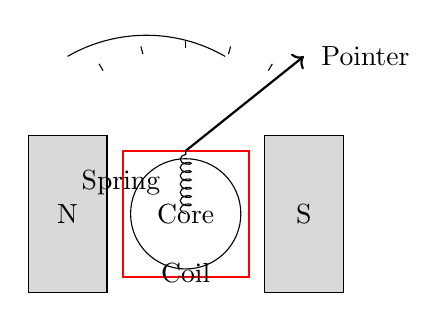
\begin{tikzpicture}
    % Magnets
    \draw [fill=gray!30] (-2, -1) rectangle (-1, 1); \node at (-1.5, 0) {N};
    \draw [fill=gray!30] (1, -1) rectangle (2, 1); \node at (1.5, 0) {S};
    % Core
    \draw (0,0) circle (0.7); \node at (0,0) {Core};
    % Coil
    \draw [thick, color=red] (-0.8, -0.8) rectangle (0.8, 0.8); \node at (0, -0.5) [below] {Coil};
    % Pointer
    \draw [thick, ->] (0, 0.8) -- (1.5, 2); \node at (1.6, 2) [right] {Pointer};
    % Scale
    \draw (0.5, 2) arc (60:120:2);
    \foreach \x in {60, 75, 90, 105, 120} \draw (\x:2.1) -- (\x:2.2);
    % Spring
    \draw [decorate, decoration={coil, segment length=3pt, amplitude=2pt}] (0,0) -- (0, 0.8); \node at (-0.2, 0.4) [left] {Spring};
\end{tikzpicture}
\captionof{figure}{PMMC Construction}
\end{center}

\begin{center}
\captionof{table}{Construction Details}
\begin{tabulary}{\linewidth}{|L|L|}
\hline
\textbf{Component} & \textbf{Description} \\ \hline
\textbf{Permanent Magnet} & Creates strong magnetic field \\ \hline
\textbf{Moving Coil} & Lightweight coil wound on aluminum frame, placed in magnetic field \\ \hline
\textbf{Springs} & Provide controlling torque and electrical connections \\ \hline
\textbf{Pointer} & Attached to coil, moves over calibrated scale \\ \hline
\textbf{Core} & Soft iron cylindrical core to concentrate magnetic flux \\ \hline
\end{tabulary}
\end{center}

\begin{itemize}
    \item \textbf{Operating Principle}: Deflecting torque $T_d = BIlN$ (B-field strength, I-current, l-length, N-turns)
    \item \textbf{Controlling Torque}: Provided by springs proportional to deflection angle ($T_c \propto \theta$)
\end{itemize}
\end{solutionbox}

\begin{mnemonicbox}
\mnemonic{MAPS-C: Magnet Acts, Pointer Shows Current}
\end{mnemonicbox}

\questionmarks{2(a)}{3}{List out different Types of errors. Explain any Two.}

\begin{solutionbox}
\begin{center}
\captionof{table}{Types of Errors}
\begin{tabulary}{\linewidth}{|L|}
\hline
\textbf{Gross Errors} \\ \hline
\textbf{Systematic Errors} \\ \hline
\textbf{Random Errors} \\ \hline
\textbf{Environmental Errors} \\ \hline
\textbf{Loading Errors} \\ \hline
\end{tabulary}
\end{center}

\textbf{Explanation}:
\begin{enumerate}
    \item \keyword{Systematic Errors}: Consistent and predictable deviations from actual value. Caused by instrument calibration, design, or method.
    \item \keyword{Random Errors}: Unpredictable variations in measurements. Caused by noise, environmental fluctuations, or observer limitations.
\end{enumerate}
\end{solutionbox}

\begin{mnemonicbox}
\mnemonic{GSREL - Good Systems Reduce Error Levels}
\end{mnemonicbox}

\questionmarks{2(b)}{4}{Draw and Explain Maxwell's bridge.}

\begin{solutionbox}
\textbf{Maxwell's Bridge} measures inductance by comparing it with a standard capacitor.

\textbf{Circuit Diagram}:
\begin{center}
\begin{circuitikz}[american, scale=0.8]
    \draw (0,3) node[left] {A} to[R, l=$R_1$] (3,5) node[above] {B} to[R, l=$R_3$] (6,3) node[right] {C};
    \draw (6,3) to[C, l=$C_4$, *-*] (4.5, 1) to[R, l=$R_4$] (3,1) node[below] {D} to[R, l=$R_2$] (0,3);
    \draw (3,1) to[L, l=$L_x$] (1.5, 2) to[R, l=$R_x$] (0,3); % Lx and Rx in one arm usually
    % Correction: Maxwell usually has Lx in arm AB? Let's follow standard
    % Standard Maxwell: 
    % Arm 1: R1 || C1  (or R4 || C4)
    % Arm 2: R2
    % Arm 3: Rx, Lx
    % Arm 4: R3
    % Let's stick to the MDX logic: R1-R3, R2-R4, Lx and C1. 
    % Re-reading MDX Description:
    % A-B: R1
    % A-D: R2
    % B-C: R3
    % C-D: R4
    % B-D: Detector (Wait, standard bridge is A-B-C-D diamond)
    % The MDX mermaid is a bit loose. Let's draw standard Maxwell Inductance-Capacitance Bridge.
    % Arm 1 (AC): R1 || C1 (Standard variable)
    % Arm 2 (AD): R2 (Fixed)
    % Arm 3 (CB): Rx + Lx (Unknown)
    % Arm 4 (DB): R3 (Fixed)
    % Let's use the one that matches typical formulas L = CR2R3
    
    \draw (0,0) coordinate (D) to[R, l=$R_2$] (0,3) coordinate (A) to[R, l=$R_1$] (3,3) coordinate (B);
    \draw (0,3) to[C, l=$C_1$,, color=blue] (3,3); % Parallel C1 to R1
    \draw (3,3) to[R, l=$R_3$] (3,0) coordinate (C);
    \draw (0,0) to[L, l=$L_x$] (1.5,0) to[R, l=$R_x$] (3,0);
    \draw (0,3) -- (-1,3) to[sV, l=AC] (-1,0) -- (0,0);
    \draw (0,1.5) to[rmeter, t=D] (3,1.5); % Detector
\end{circuitikz} 
\captionof{figure}{Maxwell's Inductance-Capacitance Bridge}
\end{center}
\textbf{Note}: The standard Maxwell bridge puts capacitor in parallel with resistance opposite to the inductor.

\begin{center}
\captionof{table}{Components}
\begin{tabulary}{\linewidth}{|L|L|}
\hline
\textbf{Component} & \textbf{Function} \\ \hline
$R_1, R_2, R_3, R_4$ & Precision resistors \\ \hline
$L_x$ & Unknown inductor with resistance $R_x$ \\ \hline
$C_1$ & Standard capacitor \\ \hline
Detector & Headphones or null indicator \\ \hline
\end{tabulary}
\end{center}

\begin{itemize}
    \item \textbf{Balance Equation}: $L_x = R_2 R_3 C_1$
    \item \textbf{Resistance Equation}: $R_x = \frac{R_2 R_3}{R_1}$
    \item \textbf{Application}: Medium Q coils ($1 < Q < 10$).
\end{itemize}
\end{solutionbox}

\begin{mnemonicbox}
\mnemonic{MBLR - Maxwell Bridge Links Resistance}
\end{mnemonicbox}

\questionmarks{2(c)}{7}{Draw and explain construction of moving iron type instruments.}

\begin{solutionbox}
\textbf{Construction Diagram}:
\begin{center}
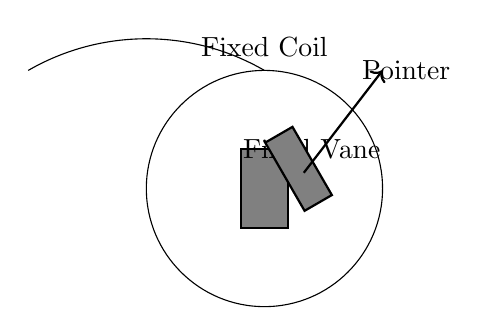
\begin{tikzpicture}
    % Coil
    \draw (0,0) circle (1.5); 
    \node at (0, 1.8) {Fixed Coil};
    
    % Fixed Vane
    \draw [thick, fill=gray] (-0.3, -0.5) rectangle (0.3, 0.5); \node at (0.6, 0.5) {Fixed Vane};
    
    % Moving Vane
    \draw [thick, fill=gray, rotate=30] (0.3, -0.5) rectangle (0.7, 0.5); 
    \draw [thick, ->] (0.5, 0.2) -- (1.5, 1.5); \node at (1.8, 1.5) {Pointer};
    
    % Scale
    \draw (0, 1.5) arc (60:120:3);
\end{tikzpicture}
\captionof{figure}{Moving Iron (Repulsion Type)}
\end{center}

\begin{center}
\captionof{table}{Construction Details}
\begin{tabulary}{\linewidth}{|L|L|}
\hline
\textbf{Component} & \textbf{Description} \\ \hline
\textbf{Coil} & Fixed coil that carries measuring current \\ \hline
\textbf{Iron Vanes} & Two soft iron pieces (one fixed, one movable) \\ \hline
\textbf{Pointer} & Attached to movable vane \\ \hline
\textbf{Control Spring} & Provides restraining torque \\ \hline
\textbf{Damping} & Air friction damping using light aluminum piston \\ \hline
\end{tabulary}
\end{center}

\begin{itemize}
    \item \textbf{Working Principle}: When current flows through coil, both iron pieces get magnetized with same polarity, causing repulsion.
    \item \textbf{Advantages}: Robust, cheap, measures AC and DC.
    \item \textbf{Disadvantages}: Non-linear scale, higher power consumption.
\end{itemize}
\end{solutionbox}

\begin{mnemonicbox}
\mnemonic{IRAM - Iron Repulsion Activates Movement}
\end{mnemonicbox}

\questionmarks{2(a) OR}{3}{Explain basic DC voltmeter.}

\begin{solutionbox}
\textbf{DC Voltmeter} consists of a PMMC meter in series with a high resistance.

\textbf{Circuit}:
\begin{center}
\begin{circuitikz}[american]
    \draw (0,0) to[R, l=$R_s$ (Multiplier)] (3,0) to[rmeter, l=$R_m$, t=PMMC] (5,0);
    \draw (0,0) to[open, v=$V_{in}$] (5,0);
\end{circuitikz}
\captionof{figure}{Basic DC Voltmeter}
\end{center}

\begin{center}
\captionof{table}{Components}
\begin{tabulary}{\linewidth}{|L|L|}
\hline
\textbf{PMMC Movement} & Basic current-sensitive movement \\ \hline
\textbf{Multiplier Resistor} & High-value series resistor to limit current \\ \hline
\textbf{Scale} & Calibrated to read voltage directly \\ \hline
\end{tabulary}
\end{center}

\begin{itemize}
    \item \textbf{Principle}: Current is proportional to voltage ($I = V / (R_s + R_m)$).
    \item \textbf{Calculation}: $R_s = \frac{V}{I_m} - R_m$.
\end{itemize}
\end{solutionbox}

\begin{mnemonicbox}
\mnemonic{SVM - Series Voltage Measurement}
\end{mnemonicbox}

\questionmarks{2(b) OR}{4}{Draw and Explain Schering bridge.}

\begin{solutionbox}
\textbf{Schering Bridge} is used for measuring capacitance and dielectric loss.

\textbf{Circuit Diagram}:
\begin{center}
\begin{circuitikz}[american, scale=0.8]
    % Arm 1: Cx (unknown)
    \draw (0,3) to[C, l=$C_1$] (1.5, 3) to[R, l=$R_1$] (3,3) coordinate (B); 
    \draw (0,0) coordinate (D) to[C, l=$C_4$] (0,3) coordinate (A);
    \draw (3,3) to[R, l=$R_3$] (3,0) coordinate (C);
    \draw (0,0) to[C, l=$C_2$] (3,0); 
    \draw (0,0.5) to[R, l=$R_2$] (3,0.5); % R2 || C2
    
    % Source and Detector
    \draw (0,3) -- (-1,3) to[sV, l=AC] (-1,0) -- (0,0);
    \draw (B) to[rmeter, t=D] (D); % Detector
\end{circuitikz}
\captionof{figure}{Schering Bridge}
\end{center}

\begin{center}
\captionof{table}{Components}
\begin{tabulary}{\linewidth}{|L|L|}
\hline
\textbf{Component} & \textbf{Function} \\ \hline
$C_1$ & Unknown capacitor (modelled with series loss $R_1$) \\ \hline
$C_2, R_2$ & Parallel RC arm \\ \hline
$R_3$ & Non-inductive resistor \\ \hline
$C_4$ & Standard loss-free capacitor \\ \hline
\end{tabulary}
\end{center}

\begin{itemize}
    \item \textbf{Balance Equations}: $C_1 = C_4 \frac{R_2}{R_3}$
    \item \textbf{Dissipation Factor}: $D = \omega C_1 R_1 = \omega C_2 R_2$
    \item \textbf{Application}: High voltage capacitor testing.
\end{itemize}
\end{solutionbox}

\begin{mnemonicbox}
\mnemonic{SCDR - Schering Capacitance Determines Resistance}
\end{mnemonicbox}

\questionmarks{2(c) OR}{7}{Write shortnote on Electronic Multimeter.}

\begin{solutionbox}
\textbf{Electronic Multimeter} uses electronic circuits (amplifiers) to drive the meter, offering high input impedance.

\textbf{Block Diagram}:
\begin{center}
\begin{tikzpicture}[node distance=1.5cm, auto]
    \node [gtu block] (Att) {Attenuator};
    \node [gtu block, left=of Att] (In) {Input};
    \node [gtu block, right=of Att] (Conv) {Converter};
    \node [gtu block, right=of Conv] (Amp) {Amplifier};
    \node [gtu block, right=of Amp] (Rect) {Rectifier};
    \node [gtu block, right=of Rect] (Disp) {Display};

    \draw [gtu arrow] (In) -- (Att);
    \draw [gtu arrow] (Att) -- (Conv);
    \draw [gtu arrow] (Conv) -- (Amp);
    \draw [gtu arrow] (Amp) -- (Rect);
    \draw [gtu arrow] (Rect) -- (Disp);
\end{tikzpicture}
\captionof{figure}{Electronic Multimeter Block Diagram}
\end{center}

\begin{center}
\captionof{table}{Features and Description}
\begin{tabulary}{\linewidth}{|L|L|}
\hline
\textbf{Feature} & \textbf{Description} \\ \hline
\textbf{Functions} & Measures Voltage, Current, Resistance (AC/DC) \\ \hline
\textbf{Sensitivity} & High (typically 10M$\Omega$ input impedance) \\ \hline
\textbf{Ranges} & Switchable ranges for wide measurement capability \\ \hline
\textbf{Accuracy} & Better than VOM (Volt-Ohm-Milliammeter) \\ \hline
\textbf{Display} & Analog (PMCC) or Digital (LCD/LED) \\ \hline
\end{tabulary}
\end{center}

\begin{itemize}
    \item \textbf{Advantages}: Minimal loading effect, reliable, compact.
\end{itemize}
\end{solutionbox}

\begin{mnemonicbox}
\mnemonic{VCAR-D: Voltage, Current And Resistance - Displayed}
\end{mnemonicbox}


\questionmarks{3(a)}{3}{Explain Various probes for CRO.}

\begin{solutionbox}
\begin{center}
\captionof{table}{Types of Probes}
\begin{tabulary}{\linewidth}{|L|L|}
\hline
\textbf{Type} & \textbf{Description} \\ \hline
\textbf{Passive Probe (1X)} & Direct connection probe with no attenuation \\ \hline
\textbf{Passive Probe (10X)} & Attenuates signal by factor of 10, reduces circuit loading \\ \hline
\textbf{Active Probe} & Contains active components (FETs) for high impedance, low capacitance \\ \hline
\textbf{Current Probe} & Measures current by sensing magnetic field (clip-on) \\ \hline
\end{tabulary}
\end{center}

\begin{itemize}
    \item \textbf{Selection Criteria}: Bandwidth, loading effect, measurement range.
    \item \textbf{Compensation}: 10X probes require adjustment to match oscilloscope input capacitance.
\end{itemize}
\end{solutionbox}

\begin{mnemonicbox}
\mnemonic{PAC-S: Probes Allow Circuit Sensing}
\end{mnemonicbox}

\questionmarks{3(b)}{4}{Draw and explain construction of Clamp on Meter.}

\begin{solutionbox}
\textbf{Clamp Meter} (Tong Tester) measures AC current without breaking the circuit.

\textbf{Construction Diagram}:
\begin{center}
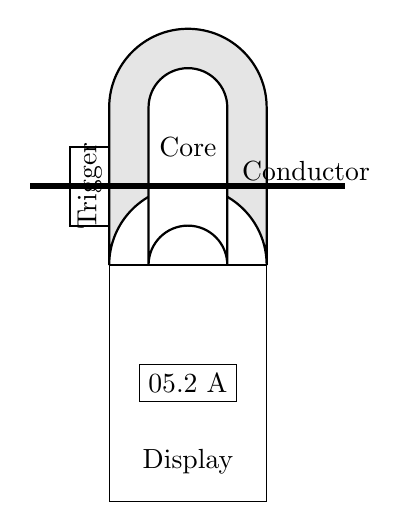
\begin{tikzpicture}
    % Clamp with core
    \draw [thick, fill=gray!20] (0,2) arc (180:0:1) -- (2,0) arc (0:180:1) -- cycle;
    \draw [thick, fill=white] (0.5,2) arc (180:0:0.5) -- (1.5,0) arc (0:180:0.5) -- cycle;
    \node at (1,1.5) {Core};
    
    % Trigger
    \draw [thick] (-0.5, 0.5) rectangle (0, 1.5); \node [rotate=90] at (-0.25, 1) {Trigger};
    
    % Body/Display
    \draw (0, -3) rectangle (2, 0);
    \node at (1, -1.5) [draw, fill=white] {05.2 A}; \node at (1, -2.5) {Display};
    
    % Wire
    \draw [line width=2pt] (-1, 1) -- (3, 1); \node at (2.5, 1.2) {Conductor};
\end{tikzpicture}
\captionof{figure}{Clamp Meter Construction}
\end{center}

\begin{center}
\captionof{table}{Components}
\begin{tabulary}{\linewidth}{|L|L|}
\hline
\textbf{Component} & \textbf{Function} \\ \hline
\textbf{Split Core CT} & Ferrite core that clamps around conductor (Primary winding is the conductor itself) \\ \hline
\textbf{Coil Winding} & Secondary winding on core that generates induced current \\ \hline
\textbf{Signal Circuitry} & Converts current to measurable signal \\ \hline
\textbf{Display Unit} & Digital/analog display calibrated in amps \\ \hline
\textbf{Trigger} & Opens/closes core jaws \\ \hline
\end{tabulary}
\end{center}

\begin{itemize}
    \item \textbf{Principle}: Current Transformer (CT). $I_s = I_p \times \frac{N_p}{N_s}$.
    \item \textbf{Application}: Measuring high current in live wires safely.
\end{itemize}
\end{solutionbox}

\begin{mnemonicbox}
\mnemonic{CAMP - Current Analyzed by Magnetic Principle}
\end{mnemonicbox}

\questionmarks{3(c)}{7}{Write shortnote on successive approximation type DVM.}

\begin{solutionbox}
\textbf{SAR DVM} uses a binary search algorithm to digitize analog voltage.

\textbf{Block Diagram}:
\begin{center}
\begin{tikzpicture}[node distance=1.5cm, auto]
    \node [gtu block] (Comp) {Comparator};
    \node [gtu block, left=of Comp] (SH) {Sample \& Hold};
    \node [gtu block, left=of SH] (In) {Input};
    \node [gtu block, right=of Comp] (SAR) {SAR Logic};
    \node [gtu block, below=of SAR] (DAC) {DAC};
    \node [gtu block, right=of SAR] (Disp) {Display};

    \draw [gtu arrow] (In) -- (SH);
    \draw [gtu arrow] (SH) -- (Comp);
    \draw [gtu arrow] (Comp) -- (SAR);
    \draw [gtu arrow] (SAR) -- (DAC);
    \draw [gtu arrow] (DAC) -| (Comp);
    \draw [gtu arrow] (SAR) -- (Disp);
\end{tikzpicture}
\captionof{figure}{Successive Approximation DVM}
\end{center}

\begin{center}
\captionof{table}{Functional Blocks}
\begin{tabulary}{\linewidth}{|L|L|}
\hline
\textbf{Block} & \textbf{Function} \\ \hline
\textbf{Sample \& Hold} & Captures and holds input voltage stable during conversion \\ \hline
\textbf{Comparator} & Compares input voltage with DAC output \\ \hline
\textbf{SAR Logic} & Sets bits from MSB to LSB. If $V_{DAC} > V_{in}$, resets bit; else keeps it \\ \hline
\textbf{DAC} & Converts digital code back to analog for comparison \\ \hline
\end{tabulary}
\end{center}

\begin{itemize}
    \item \textbf{Conversion Time}: Fixed ($n$ clock cycles for $n$-bit). $T = n \times T_{clk}$.
    \item \textbf{Advantages}: Moderate speed (faster than dual slope), constant conversion time.
\end{itemize}
\end{solutionbox}

\begin{mnemonicbox}
\mnemonic{SACD - Sample, Approximate, Compare, Display}
\end{mnemonicbox}

\questionmarks{3(a) OR}{3}{Explain PH Sensor.}

\begin{solutionbox}
\textbf{pH Sensor} measures the acidity or alkalinity of a solution.

\textbf{Diagram}:
\begin{center}
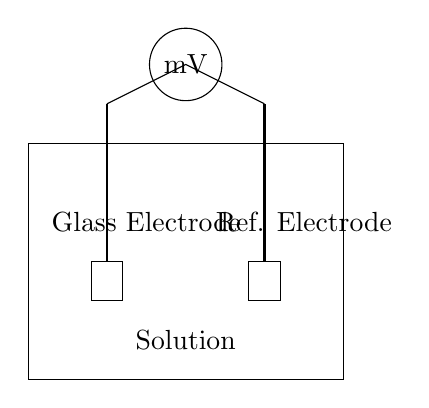
\begin{tikzpicture}
    % Beaker
    \draw (0,0) -- (0,3) -- (4,3) -- (4,0) -- cycle; \node at (2,0.5) {Solution};
    
    % Electrodes
    \draw [thick] (1,3.5) -- (1,1); \draw [fill=white] (0.8,1) rectangle (1.2,1.5); \node at (1.5, 2) {Glass Electrode};
    \draw [thick] (3,3.5) -- (3,1); \draw [fill=white] (2.8,1) rectangle (3.2,1.5); \node at (3.5, 2) {Ref. Electrode};
    
    % Meter
    \draw (1,3.5) -- (2,4) -- (3,3.5);
    \node [draw, circle] at (2,4) {mV};
\end{tikzpicture}
\captionof{figure}{pH Measurement System}
\end{center}

\begin{itemize}
    \item \textbf{Glass Electrode}: Sensitive to $H^+$ ion concentration.
    \item \textbf{Reference Electrode}: Provides stable potential (Ag/AgCl).
    \item \textbf{Nernst Equation}: $E = E_0 - \frac{kT}{nF} \ln[H^+]$.
    \item \textbf{Output}: Approx 59mV change per pH unit at 25$^\circ$C.
\end{itemize}
\end{solutionbox}

\begin{mnemonicbox}
\mnemonic{PHRV - PH Related to Voltage}
\end{mnemonicbox}

\questionmarks{3(b) OR}{4}{Draw and explain construction of Electronic Watt Meter.}

\begin{solutionbox}
\textbf{Electronic Wattmeter} measures power ($P = VI \cos \phi$).

\textbf{Block Diagram}:
\begin{center}
\begin{tikzpicture}[node distance=1.5cm, auto]
    \node [gtu block] (Mult) {Multiplier};
    \node [gtu block, left=of Mult, yshift=1cm] (VS) {Voltage Sensor};
    \node [gtu block, left=of Mult, yshift=-1cm] (CS) {Current Sensor};
    \node [gtu block, right=of Mult] (Int) {Integrator/Avg};
    \node [gtu block, right=of Int] (Disp) {Display};

    \draw [gtu arrow] (VS) -- (Mult);
    \draw [gtu arrow] (CS) -- (Mult);
    \draw [gtu arrow] (Mult) -- (Int);
    \draw [gtu arrow] (Int) -- (Disp);
    
    \node [left=of VS] (V) {Line V}; \draw [gtu arrow] (V) -- (VS);
    \node [left=of CS] (I) {Load I}; \draw [gtu arrow] (I) -- (CS);
\end{tikzpicture}
\captionof{figure}{Electronic Wattmeter}
\end{center}

\begin{itemize}
    \item \textbf{Multiplier}: Produces instantaneous power signal $p(t) = v(t) \times i(t)$.
    \item \textbf{Integrator/Averager}: Averagers the instantaneous power to get true power $P_{avg}$.
    \item \textbf{Display}: Shows value in Watts.
\end{itemize}
\end{solutionbox}

\begin{mnemonicbox}
\mnemonic{VIMP - Voltage \& Intensity Make Power}
\end{mnemonicbox}

\questionmarks{3(c) OR}{7}{Write shortnote on Integrating type DVM.}

\begin{solutionbox}
\textbf{Integrating DVM} measures true average value of input voltage over a fixed period. Example: Dual-Slope Integrating DVM.

\textbf{Block Diagram}:
\begin{center}
\begin{tikzpicture}[node distance=1.5cm, auto]
    \node [gtu block] (Int) {Integrator};
    \node [gtu block, left=of Int] (Sw) {Switch};
    \node [gtu block, right=of Int] (Comp) {Comparator};
    \node [gtu block, right=of Comp] (Logic) {Control Logic};
    \node [gtu block, below=of Logic] (Count) {Counter};
    \node [gtu block, right=of Logic] (Disp) {Display};
    \node [gtu block, below=of Int] (Vref) {$V_{ref}$};
    
    \draw [gtu arrow] (Sw) -- (Int);
    \draw [gtu arrow] (Int) -- (Comp);
    \draw [gtu arrow] (Comp) -- (Logic);
    \draw [gtu arrow] (Logic) -- (Count);
    \draw [gtu arrow] (Count) -- (Disp);
    \draw [gtu arrow] (Logic) -| (Sw);
    \draw [gtu arrow] (Vref) -| (Sw);
\end{tikzpicture}
\captionof{figure}{Dual Slope DVM}
\end{center}

\begin{center}
\captionof{table}{Phases}
\begin{tabulary}{\linewidth}{|L|L|}
\hline
\textbf{Phase 1 (Signal Integration)} & Integrate $V_{in}$ for fixed time $T_1$. Capacitor charges. \\ \hline
\textbf{Phase 2 (Reference Integration)} & Integrate fixed $-V_{ref}$. Capacitor discharges to zero. Measure time $T_2$. \\ \hline
\end{tabulary}
\end{center}

\begin{itemize}
    \item \textbf{Principle}: $V_{in} = V_{ref} \times \frac{T_2}{T_1}$.
    \item \textbf{Features}: Excellent noise rejection (averages out noise), high accuracy, slower speed.
\end{itemize}
\end{solutionbox}

\begin{mnemonicbox}
\mnemonic{TINA - Time Integration Nullifies Average}
\end{mnemonicbox}

\questionmarks{4(a)}{3}{Write advantages and applications of Digital storage oscilloscope.}

\begin{solutionbox}
\begin{center}
\captionof{table}{Advantages and Applications}
\begin{tabulary}{\linewidth}{|L|L|}
\hline
\textbf{Advantages} & \textbf{Applications} \\ \hline
Pre-trigger Viewing & Capturing transient events \\ \hline
Infinite Storage & Analyzing intermittent faults \\ \hline
Waveform Processing (FFT, Math) & Complex signal analysis \\ \hline
Hard Copy/PC Interface & Data logging and documentation \\ \hline
\end{tabulary}
\end{center}
\end{solutionbox}

\begin{mnemonicbox}
\mnemonic{SPADE - Storage, Processing, Analysis, Display, Events}
\end{mnemonicbox}

\questionmarks{4(b)}{4}{Write shortnote on Electronic Energy Meter.}

\begin{solutionbox}
\textbf{Electronic Energy Meter} measures energy consumption in kWh using digital circuits.

\textbf{Block Diagram}:
\begin{center}
\begin{tikzpicture}[node distance=1.5cm, auto]
    \node [gtu block] (P) {Power CPU (Multiplier)};
    \node [gtu block, left=of P] (Sens) {V \& I Sensors};
    \node [gtu block, right=of P] (Mic) {Microcontroller};
    \node [gtu block, right=of Mic] (Disp) {LCD};
    \node [gtu block, below=of P] (Pulse) {Pulse LED};

    \draw [gtu arrow] (Sens) -- (P);
    \draw [gtu arrow] (P) -- (Mic);
    \draw [gtu arrow] (Mic) -- (Disp);
    \draw [gtu arrow] (P) -- (Pulse);
\end{tikzpicture}
\captionof{figure}{Energy Meter System}
\end{center}

\begin{itemize}
    \item \textbf{Sensors}: Resistive divider for Voltage, Shunt/CT for Current.
    \item \textbf{Metering IC}: Multiplies V and I to get power, converts to frequency (pulses).
    \item \textbf{Microcontroller}: Accumulates pulses to calculate Energy ($\int P dt$).
    \item \textbf{Display}: Shows total kWh.
\end{itemize}
\end{solutionbox}

\begin{mnemonicbox}
\mnemonic{VICES - Voltage \& Current Energy Summation}
\end{mnemonicbox}

\questionmarks{4(c)}{7}{Draw and explain Block diagram of Analog C.R.O. and working of each block in brief.}

\begin{solutionbox}
\textbf{Block Diagram}:
\begin{center}
\begin{tikzpicture}[node distance=1.5cm, auto]
    \node [gtu block] (V_Amp) {Vertical Amp};
    \node [gtu block, left=of V_Amp] (In) {Input};
    \node [gtu block, right=of V_Amp] (Delay) {Delay Line};
    \node [gtu block, below=of V_Amp] (Trig) {Trigger};
    \node [gtu block, right=of Trig] (TB) {Time Base};
    \node [gtu block, right=of TB] (H_Amp) {Horiz Amp};
    \node [gtu block, right=of Delay] (CRT) {CRT};
    \node [gtu block, below=of Trig] (PS) {Power Supply};

    \draw [gtu arrow] (In) -- (V_Amp);
    \draw [gtu arrow] (V_Amp) -- (Delay);
    \draw [gtu arrow] (Delay) -- node[above]{Y} (CRT);
    \draw [gtu arrow] (V_Amp) -- (Trig);
    \draw [gtu arrow] (Trig) -- (TB);
    \draw [gtu arrow] (TB) -- (H_Amp);
    \draw [gtu arrow] (H_Amp) -- node[right]{X} (CRT);
    \draw [gtu arrow] (PS) -| (CRT);
\end{tikzpicture}
\captionof{figure}{CRO Block Diagram}
\end{center}

\begin{center}
\captionof{table}{Block Functions}
\begin{tabulary}{\linewidth}{|L|L|}
\hline
\textbf{Block} & \textbf{Function} \\ \hline
\textbf{Vertical Amplifier} & Amplifies weak input signals for Y-deflection \\ \hline
\textbf{Delay Line} & Delays signal to Y-plates to allow sweep to start \\ \hline
\textbf{Trigger Circuit} & Synchronizes sweep with input signal for stable display \\ \hline
\textbf{Time Base} & Generates sawtooth wave for X-deflection (sweep) \\ \hline
\textbf{Horizontal Amplifier} & Amplifies sawtooth wave for X-plates \\ \hline
\textbf{CRT} & Displays waveform (Electron gun, Deflection system, Screen) \\ \hline
\end{tabulary}
\end{center}
\end{solutionbox}

\begin{mnemonicbox}
\mnemonic{VTHCP - Vertical, Time, Horizontal, CRT, Power}
\end{mnemonicbox}

\questionmarks{4(a) OR}{3}{Draw and explain PIEZO-ELECTRIC transducer.}

\begin{solutionbox}
\textbf{Piezoelectric Transducer} is an active transducer converting pressure to voltage.

\textbf{Diagram}:
\begin{center}
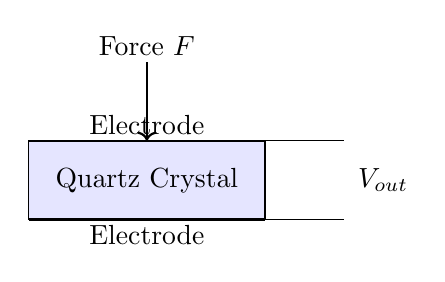
\begin{tikzpicture}
    % Crystal
    \draw [fill=blue!10] (0,0) rectangle (3,1); \node at (1.5,0.5) {Quartz Crystal};
    % Electrodes
    \draw [thick] (0,1) -- (3,1); \node at (1.5,1.2) {Electrode};
    \draw [thick] (0,0) -- (3,0); \node at (1.5,-0.2) {Electrode};
    % Force
    \draw [->, thick] (1.5, 2) -- (1.5, 1); \node at (1.5, 2.2) {Force $F$};
    % Output
    \draw (3,1) -- (4,1); \draw (3,0) -- (4,0);
    \node at (4.5, 0.5) {$V_{out}$};
\end{tikzpicture}
\captionof{figure}{Piezoelectric Crystal}
\end{center}

\begin{itemize}
    \item \textbf{Principle}: Piezoelectric Effect. Stress $\rightarrow$ Charge.
    \item \textbf{Materials}: Quartz, Rochelle Salt, PZT.
    \item \textbf{Output}: $V = g \cdot t \cdot P$ ($P=Pressure$, $t=thickness$, $g=voltage sensitivity$).
    \item \textbf{Application}: Dynamic pressure, Accelerometers.
\end{itemize}
\end{solutionbox}

\begin{mnemonicbox}
\mnemonic{PFVD - Pressure Forms Voltage via Displacement}
\end{mnemonicbox}

\questionmarks{4(b) OR}{4}{Draw and explain Measurement of Frequency by using CRO.}

\begin{solutionbox}
\textbf{Method 1: Time Base (Direct)}
\begin{itemize}
    \item Measure Time Period $T$ of one cycle on screen.
    \item Calculate $f = 1/T$.
\end{itemize}

\textbf{Method 2: Lissajous Figures (XY Mode)}
\begin{center}
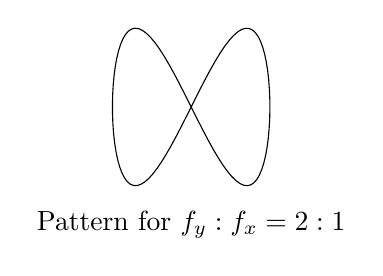
\begin{tikzpicture}
    % Figure 8
    \draw [domain=0:360, samples=100] plot ({sin(\x)}, {sin(2*\x)});
    \node at (0,-1.5) {Pattern for $f_y : f_x = 2:1$};
\end{tikzpicture}
\captionof{figure}{Lissajous Pattern Example}
\end{center}

\begin{itemize}
    \item Apply unknown $f_y$ to Y and standard $f_x$ to X.
    \item $\frac{f_y}{f_x} = \frac{\text{Number of horizontal tangents}}{\text{Number of vertical tangents}}$
\end{itemize}
\end{solutionbox}

\begin{mnemonicbox}
\mnemonic{LTX - Lissajous or Time for X-axis}
\end{mnemonicbox}

\questionmarks{4(c) OR}{7}{Draw and explain Thermistor and Thermocouple.}

\begin{solutionbox}
\textbf{1. Thermistor}:
Variable resistor sensitive to temperature.
\begin{itemize}
    \item \textbf{Types}: NTC (Negative Temp Coeff) - R decreases as T increases (most common). PTC - R increases.
    \item \textbf{Characteristic}: Highly sensitive, non-linear.
\end{itemize}

\textbf{2. Thermocouple}:
Active transducer based on Seebeck Effect.
\begin{center}
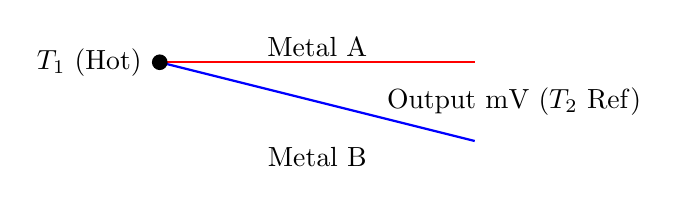
\begin{tikzpicture}
    \draw [thick, red] (0,0) -- (4,0); \node at (2, 0.2) {Metal A};
    \draw [thick, blue] (0,0) -- (4, -1); \node at (2, -1.2) {Metal B};
    \node [circle, fill, inner sep=2pt, label=left:$T_1$ (Hot)] at (0,0) {};
    \node at (4.5, -0.5) {Output mV ($T_2$ Ref)};
\end{tikzpicture}
\captionof{figure}{Thermocouple}
\end{center}
\begin{itemize}
    \item \textbf{Principle}: Junction of dissimilar metals at different temperatures generates EMF.
    \item \textbf{Types}: J (Iron-Constantan), K (Chromel-Alumel).
    \item \textbf{Range}: Wide temperature range, robust.
\end{itemize}
\end{solutionbox}

\begin{mnemonicbox}
\mnemonic{TRT/TVJ - Temperature Resistance/Voltage Junction}
\end{mnemonicbox}

\questionmarks{5(a)}{3}{Draw and Explain Velocity transducer.}

\begin{solutionbox}
\textbf{Electromagnetic Velocity Transducer} (Moving coil type).

\textbf{Diagram}:
\begin{center}
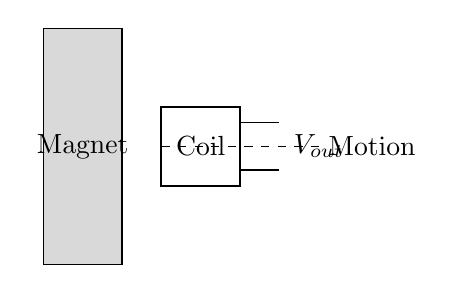
\begin{tikzpicture}
    % Magnet
    \draw [fill=gray!30] (0,0) rectangle (1,3); \node at (0.5, 1.5) {Magnet};
    % Coil
    \draw [thick] (1.5, 1) rectangle (2.5, 2); \node at (2, 1.5) {Coil};
    \draw [dashed] (1.5, 1.5) -- (3.5, 1.5) node[right]{Motion};
    % Terminals
    \draw (2.5, 1.8) -- (3, 1.8);
    \draw (2.5, 1.2) -- (3, 1.2); \node at (3.5, 1.5) {$V_{out}$};
\end{tikzpicture}
\captionof{figure}{Velocity Transducer}
\end{center}

\begin{itemize}
    \item \textbf{Principle}: Faraday's Law ($e = N \frac{d\phi}{dt}$). Since $\frac{d\phi}{dt} \propto \text{velocity}$.
    \item \textbf{Output}: Voltage is directly proportional to linear velocity of coil relative to magnet.
    \item \textbf{Application}: Vibration monitoring.
\end{itemize}
\end{solutionbox}

\begin{mnemonicbox}
\mnemonic{VMMF - Velocity Makes Magnetic Flux}
\end{mnemonicbox}

\questionmarks{5(b)}{4}{Give Classification of transducers and explain it.}

\begin{solutionbox}
\begin{center}
\captionof{table}{Classification}
\begin{tabulary}{\linewidth}{|L|L|}
\hline
\textbf{Basis} & \textbf{Types} \\ \hline
\textbf{Power Source} & \textbf{Active}: Self-generating (Thermocouple, Piezo). \textbf{Passive}: External power required (RTD, LVDT). \\ \hline
\textbf{Transduction} & Resistive, Inductive, Capacitive, etc. \\ \hline
\textbf{Function} & \textbf{Primary}: Detects phenomenon (Bourdon tube). \textbf{Secondary}: Converts to electrical (LVDT). \\ \hline
\textbf{Output} & Analog vs Digital. \\ \hline
\end{tabulary}
\end{center}
\end{solutionbox}

\begin{mnemonicbox}
\mnemonic{APRCI - Active Passive Resistive Capacitive Inductive}
\end{mnemonicbox}

\questionmarks{5(c)}{7}{Write shortnote on LVDT.}

\begin{solutionbox}
\textbf{LVDT (Linear Variable Differential Transformer)} is an inductive transducer for displacement.

\textbf{Diagram}:
\begin{center}
\begin{circuitikz}[scale=0.8]
    % Core
    \draw [fill=gray!20] (2, 2.5) rectangle (4, 3.5); \node at (3,3) {Core};
    \draw [->] (3, 3.6) -- (4, 3.6) node[right]{Displacement};
    
    % Primary
    \draw (1, 2) to[L, l=Primary] (1,4);
    
    % Secondaries
    \draw (5, 4.5) to[L, l=$S_1$] (5, 3.5);
    \draw (5, 2.5) to[L, l=$S_2$] (5, 1.5);
    
    % Connections (Series Opposing)
    \draw (5, 3.5) -- (5, 2.5); % Connect distinct
    % Actually typically S1 end connects to S2 end.
    % Let's draw schematic style
\end{circuitikz}
\end{center}
\textbf{Schematic}:
\begin{center}
\begin{circuitikz}
    \draw (0,0) node[left]{Excitation} to[L, l=$P$] (0,2);
    \draw (2,2) to[L, l=$S_1$] (2,1) -- (2,0.5);
    \draw (2,-0.5) -- (2,-1) to[L, l=$S_2$] (2,-2);
    \draw (2,1) -- (3,1) node[right]{Output +};
    \draw (2,-2) -- (3,-2) node[right]{Output -};
    \draw (2,0.5) -- (2,-0.5); % Series connection? 
    % Series Opposition: Vout = Vs1 - Vs2.
    % Connect bottom of S1 to bottom of S2? Or Top of S2?
    % Usually: S1_dot -- S2_dot. 
    \node at (1,0) {Core coupling};
\end{circuitikz}
\captionof{figure}{LVDT Schematic}
\end{center}

\begin{itemize}
    \item \textbf{Construction}: One primary winding, two secondary windings connected in \keyword{series opposition}. Movable soft iron core.
    \item \textbf{Working}:
    \begin{itemize}
        \item Null Position: Voltages in $S_1$ and $S_2$ equal and cancel out ($V_{out}=0$).
        \item Displacement: Core movement changes flux coupling, creating differential output ($V_{out} = V_{s1} - V_{s2}$).
    \end{itemize}
    \item \textbf{Advantages}: Linearity, infinite resolution, rugged.
\end{itemize}
\end{solutionbox}

\begin{mnemonicbox}
\mnemonic{CPSO: Core Position Shifts Output}
\end{mnemonicbox}

\questionmarks{5(a) OR}{3}{Draw and Explain block diagram of simple frequency Counter.}

\begin{solutionbox}
\textbf{Digital Frequency Counter} counts pulses over a fixed time measuring frequency ($f = N/t$).

\textbf{Block Diagram}:
\begin{center}
\begin{tikzpicture}[node distance=1.5cm, auto]
    \node [gtu block] (Gate) {Main Gate};
    \node [gtu block, left=of Gate] (In) {Input};
    \node [gtu block, below=of Gate] (TB) {Time Base};
    \node [gtu block, right=of Gate] (Count) {Counter};
    \node [gtu block, right=of Count] (Disp) {Display};

    \draw [gtu arrow] (In) -- (Gate);
    \draw [gtu arrow] (TB) -- (Gate);
    \draw [gtu arrow] (Gate) -- (Count);
    \draw [gtu arrow] (Count) -- (Disp);
\end{tikzpicture}
\captionof{figure}{Frequency Counter}
\end{center}

\begin{itemize}
    \item \textbf{Time Base}: Generates precise "Gate" signal (e.g., 1 sec).
    \item \textbf{Main Gate}: Allows input pulses to pass only for gate duration.
    \item \textbf{Counter}: Counts pulses. Reading represents frequency.
\end{itemize}
\end{solutionbox}

\begin{mnemonicbox}
\mnemonic{IGTCD - Input Gated Time Counts Display}
\end{mnemonicbox}

\questionmarks{5(b) OR}{4}{Draw and Explain Capacitive Transducer.}

\begin{solutionbox}
\textbf{Capacitive Transducer} works on $C = \frac{\epsilon A}{d}$.

\textbf{Principles}:
\begin{enumerate}
    \item \textbf{Variable Separation ($d$)}: Moving plate changes distance. Used for pressure/displacement.
    \item \textbf{Variable Area ($A$)}: Overlapping area changes.
    \item \textbf{Variable Dielectric ($\epsilon$)}: Dielectric moves between plates.
\end{enumerate}

\textbf{Diagram}:
\begin{center}
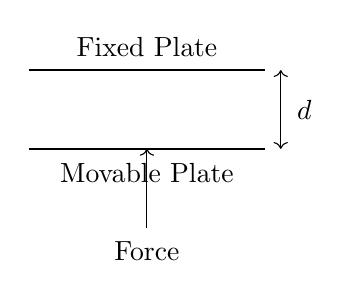
\begin{tikzpicture}
    \draw [thick] (0,2) -- (3,2); \node at (1.5, 2.3) {Fixed Plate};
    \draw [thick] (0,1) -- (3,1); \node at (1.5, 0.7) {Movable Plate};
    \draw [<->] (3.2, 1) -- (3.2, 2); \node at (3.5, 1.5) {$d$};
    \draw [->] (1.5, 0) -- (1.5, 1); \node at (1.5, -0.3) {Force};
\end{tikzpicture}
\captionof{figure}{Variable Gap Capacitive Transducer}
\end{center}
\end{solutionbox}

\begin{mnemonicbox}
\mnemonic{CGAD - Capacitance Gap Area Dielectric}
\end{mnemonicbox}

\questionmarks{5(c) OR}{7}{Draw and Explain block diagram of Function generator.}

\begin{solutionbox}
\textbf{Function Generator} produces Sine, Square, and Triangular waves over wide frequency range.

\textbf{Block Diagram}:
\begin{center}
\begin{tikzpicture}[node distance=1.5cm, auto]
    \node [gtu block] (Osc) {Oscillator / Current Source};
    \node [gtu block, right=of Osc] (Tri) {Triangle Gen};
    \node [gtu block, right=of Tri] (Shape) {Sine Shaper};
    \node [gtu block, below=of Tri] (Comp) {Comparator};
    \node [gtu block, right=of Shape, xshift=1cm] (Amp) {Output Amp};
    
    \draw [gtu arrow] (Osc) -- (Tri);
    \draw [gtu arrow] (Tri) -- (Shape);
    \draw [gtu arrow] (Tri) -- (Comp);
    \draw [gtu arrow] (Comp) -| (Osc); % Feedback
    
    % Switch
    \node [right=of Tri, yshift=1cm] (Sw) {Switch}; 
    \draw [dashed] (Tri) -- (Amp);
    \draw [dashed] (Shape) -- (Amp);
    \draw [dashed] (Comp.east) -- ++(0.5,0) |- (Amp);
    
\end{tikzpicture}
\captionof{figure}{Function Generator}
\end{center}

\begin{center}
\captionof{table}{Working}
\begin{tabulary}{\linewidth}{|L|L|}
\hline
\textbf{Frequency Control} & Varies current to integrating capacitor \\ \hline
\textbf{Triangle} & Basic waveform generated by constant current charging/discharging \\ \hline
\textbf{Comparator} & Switches current direction, generates Square wave \\ \hline
\textbf{Sine Shaper} & Networks convert triangle to sine \\ \hline
\textbf{Output Amplifier} & Sets amplitude and impedance \\ \hline
\end{tabulary}
\end{center}
\end{solutionbox}

\begin{mnemonicbox}
\mnemonic{FWMASO - Frequency Waveform Mode Amplitude Sweep Output}
\end{mnemonicbox}

\end{document}
